\documentclass{article}
\usepackage{graphicx} %Uncomment this line when you want pictures!
\usepackage[export]{adjustbox}

\title{Homework 1 CSCI 451}
\author{Nicholas Rust}
\date{due: 12 September 2019}

\begin{document}
\maketitle

\begin{enumerate}
	\item
	\begin{itemize}
		\item Yes you can visit a gene bank and check a number of protein sequences.
		\item The MET is the first amino acid.
	\end{itemize}
	\item There are usually 2 copies of nuclear DNA in a eukariotic cell. There are between 100 and 1000 copies of mitochondrial DNA in a eukariotic cell, about 500 per human cell.
	\item Genes are currently supposed to be somewhat randomly distributed throughout the genome, however, there are theories that some groups are clumped together rather than completey randomly distributed.
	\item It is mentioned that there is a codon bias for D. \em{melanogaster}\em where the more commonly expressed genes use the more readily available codons in the cell. This does not appear to be true for most organisms.
	\item ATG is the start translation sequence, so ACTTGTC is the 5' UTR. TAG is the end sequence used here, meaning the 3' UTR is GTCATG. 
\end{enumerate}

\begin{figure}
    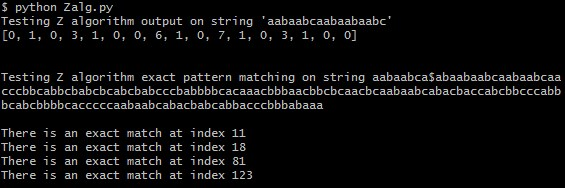
\includegraphics[width=1.2\textwidth,center]{output.jpg}
    \caption{Z Algorithm Output}
\end{figure}


\end{document}